% Krydo on Stellar — Business Plan & Stellar Garage Delhi Residency
% Compile: pdflatex krydo-stellar-business-plan.tex (run twice for TOC)
\documentclass[11pt,a4paper]{article}

% ── Encoding & fonts ─────────────────────────────────────────────────────────
\usepackage[utf8]{inputenc}
\usepackage[T1]{fontenc}
\usepackage{lmodern}
\usepackage{microtype}

% ── Layout ───────────────────────────────────────────────────────────────────
\usepackage[
  top=2.4cm,
  bottom=2.4cm,
  left=2.6cm,
  right=2.6cm,
  headheight=14pt
]{geometry}
\usepackage{parskip}
\setlength{\parindent}{0pt}

% ── Graphics & colour ────────────────────────────────────────────────────────
\usepackage{xcolor}
\definecolor{StellarBlue}{HTML}{14B6E7}
\definecolor{StellarDark}{HTML}{0B3D4C}
\definecolor{AccentGold}{HTML}{C9A227}
\definecolor{BodyGray}{HTML}{374151}
\definecolor{LightBg}{HTML}{F3F7FA}
\definecolor{TableHead}{HTML}{0F2B36}

\usepackage{tikz}
\usetikzlibrary{calc, positioning, shapes.geometric, arrows.meta}

% ── Tables & lists ───────────────────────────────────────────────────────────
\usepackage{booktabs}
\usepackage{tabularx}
\usepackage{array}
\usepackage{longtable}
\usepackage{enumitem}
\setlist[itemize]{leftmargin=1.4em, itemsep=2pt, topsep=4pt}
\setlist[enumerate]{leftmargin=1.6em, itemsep=2pt, topsep=4pt}

% ── Boxes & headers ──────────────────────────────────────────────────────────
\usepackage{tcolorbox}
\tcbuselibrary{skins,breakable}
\newtcolorbox{keybox}[1][]{
  enhanced,
  breakable,
  colback=LightBg,
  colframe=StellarBlue,
  boxrule=0.6pt,
  arc=2pt,
  left=8pt, right=8pt, top=6pt, bottom=6pt,
  fonttitle=\bfseries\color{StellarDark},
  title=#1
}
\newtcolorbox{warningbox}[1][]{
  enhanced,
  breakable,
  colback=AccentGold!8,
  colframe=AccentGold!80,
  boxrule=0.6pt,
  arc=2pt,
  left=8pt, right=8pt, top=6pt, bottom=6pt,
  fonttitle=\bfseries,
  title=#1
}

\usepackage{titlesec}
\titleformat{\section}
  {\Large\bfseries\color{StellarDark}}
  {\thesection}{0.8em}{}[\titlerule]
\titleformat{\subsection}
  {\large\bfseries\color{StellarDark}}
  {\thesubsection}{0.6em}{}
\titlespacing*{\section}{0pt}{18pt}{8pt}
\titlespacing*{\subsection}{0pt}{12pt}{6pt}

\usepackage{fancyhdr}
\pagestyle{fancy}
\fancyhf{}
\fancyhead[L]{\small\color{BodyGray}\textsf{Krydo on Stellar --- Business Plan}}
\fancyhead[R]{\small\color{BodyGray}\textsf{Stellar Garage Delhi 2026}}
\fancyfoot[C]{\small\color{BodyGray}\thepage}
\renewcommand{\headrulewidth}{0.4pt}
\renewcommand{\footrulewidth}{0pt}

% ── Links ────────────────────────────────────────────────────────────────────
\usepackage[hidelinks,colorlinks=false]{hyperref}
\usepackage{cleveref}

% ── Misc ─────────────────────────────────────────────────────────────────────
\usepackage{graphicx}
\usepackage{float}
\usepackage{multicol}

% ── Custom commands ──────────────────────────────────────────────────────────
\newcommand{\krydo}{\textsf{Krydo}}
\newcommand{\stellar}{\textsf{Stellar}}
\newcommand{\soroban}{\textsf{Soroban}}
\newcommand{\inr}[1]{INR\,#1}
\newcommand{\highlight}[1]{\textbf{\color{StellarDark}#1}}

% ═════════════════════════════════════════════════════════════════════════════
\begin{document}

% ── Cover page ───────────────────────────────────────────────────────────────
\begin{titlepage}
  \begin{tikzpicture}[remember picture, overlay]
    \fill[StellarDark] (current page.north west) rectangle ([yshift=-7.2cm]current page.north east);
    \fill[StellarBlue] ([yshift=-7.2cm]current page.north west) rectangle ([yshift=-7.55cm]current page.north east);
    \node[anchor=north west, text=white] at ([xshift=2.6cm, yshift=-2.2cm]current page.north west) {
      \begin{minipage}{0.85\textwidth}
        {\fontsize{34}{38}\selectfont\bfseries Krydo}\\[0.35em]
        {\fontsize{16}{20}\selectfont Privacy-Preserving Financial Trust Infrastructure}\\[1.4em]
        {\fontsize{22}{26}\selectfont\bfseries Business Plan \& Technical Strategy}\\[0.5em]
        {\fontsize{13}{16}\selectfont Stellar Build Station Delhi \textbar\ 21-Day Residency}
      \end{minipage}
    };
    \node[anchor=south east, text=AccentGold!90!white] at ([xshift=-2.6cm, yshift=-6.4cm]current page.north east) {
      \begin{minipage}{0.45\textwidth}
        \raggedleft
        {\small\textsf{Powered by Rise In}}\\[0.2em]
        {\small stellar.org \textbar\ risein.com}
      \end{minipage}
    };
  \end{tikzpicture}

  \vspace*{7.8cm}

  \begin{center}
    \begin{minipage}{0.82\textwidth}
      \renewcommand{\arraystretch}{1.35}
      \begin{tabular}{@{}>{\bfseries\color{StellarDark}}p{3.2cm} p{9.5cm}@{}}
        \toprule
        Program & Stellar Build Station Delhi \\
        Organisers & Stellar \& Rise In \\
        Location & Innov8 CP, Delhi NCR \\
        Duration & 21 Days (4 July -- 25 July 2026) \\
        Cohort & 15 Selected Teams \\
        Format & Hybrid with Weekly In-Person Check-ins \\
        Build Hours & 11:00 AM -- 4:30 PM \\
        \bottomrule
      \end{tabular}
    \end{minipage}

    \vspace{2.2cm}

    {\large\color{BodyGray}
      \textit{Prove you qualify --- without revealing what you have.}\\[0.8em]
      Confidential Business Document \textbar\ July 2026
    }
  \end{center}

  \vfill
  {\small\color{BodyGray}
    Document version 1.0 \textbar\
    Prepared for Stellar Garage Delhi residency submission and investor discussions.
  }
\end{titlepage}

% ── Table of contents ────────────────────────────────────────────────────────
\tableofcontents
\newpage

% ═════════════════════════════════════════════════════════════════════════════
\section{Executive Summary}

\krydo{} is a \highlight{privacy-preserving verifiable credential platform} that enables users to prove financial and identity predicates---such as \emph{``credit score $\geq$ 700''} or \emph{``annual income $\geq$ INR\,10\,Lakh''}---\textbf{without disclosing the underlying values}. Built on zero-knowledge sigma protocols over Pedersen commitments, \krydo{} addresses a critical gap in India's rapidly evolving compliance landscape: verification flows that over-collect personal data by default.

This document outlines the business strategy, revenue model, go-to-market plan, and technical roadmap for deploying \krydo{} on the \stellar{} network as part of the \textbf{Stellar Garage Delhi} 21-day residency program.

\begin{keybox}[Strategic Thesis]
  \begin{itemize}
    \item \textbf{Problem:} Lenders, landlords, and fintechs receive full salary slips, bank statements, and PAN data when they only need a yes/no qualification answer.
    \item \textbf{Solution:} \krydo{} anchors credential trust on-chain; users generate ZK proofs in-browser; verifiers learn predicates, not PII.
    \item \textbf{Why \stellar{}:} Sub-cent transaction costs, Soroban smart contracts, cross-border settlement, and ecosystem support via Rise In sponsorship for mainnet deployment.
    \item \textbf{Business model:} B2B SaaS and per-verification API fees charged to \emph{verifiers} (NBFCs, fintechs, exchanges) and \emph{issuers} (employers, KYC providers).
    \item \textbf{Near-term goal:} Deliver a mainnet-ready demo by 25 July 2026; secure one paid pilot within 90 days post-residency.
  \end{itemize}
\end{keybox}

% ═════════════════════════════════════════════════════════════════════════════
\section{The Problem}

\subsection{Over-Collection Is the Default}

Current identity and financial verification in India follows a destructive pattern. When a lender asks \emph{``Does this applicant earn at least INR\,10\,Lakh per annum?''}, the typical response involves:

\begin{itemize}
  \item Full salary slips and employer details
  \item Six months of bank statements
  \item PAN, Aadhaar-linked KYC documents
  \item Credit bureau reports with complete score history
\end{itemize}

This data is stored indefinitely by multiple parties, re-sold through data brokers, and cannot be revoked once leaked. Under India's \textbf{Digital Personal Data Protection Act (DPDP)}, data minimisation is shifting from best practice to legal requirement.

\subsection{Why Existing Solutions Fall Short}

\begin{table}[H]
  \centering
  \caption{Competitive landscape and \krydo{} differentiation}
  \renewcommand{\arraystretch}{1.25}
  \begin{tabularx}{\textwidth}{@{}>{\bfseries}p{2.8cm} X X@{}}
    \toprule
    Approach & Limitation & \krydo{} Advantage \\
    \midrule
    Traditional KYC (Signzy, IDfy, HyperVerge) & Stores full PII; breach liability; poor revocation & Predicate-only verification; on-chain revocation \\
    Manual document upload & Slow, fraud-prone, poor UX & Cryptographic proof in milliseconds \\
    SNARK-based ZK systems & Trusted setup, circuit compilation, high gas & Sigma protocols: no setup ceremony, browser-native proofs \\
    Self-attested claims & No trust anchor & On-chain issuer whitelist + credential anchoring \\
    \bottomrule
  \end{tabularx}
\end{table}

% ═════════════════════════════════════════════════════════════════════════════
\section{Product Overview: \krydo{}}

\subsection{Value Proposition}

\krydo{} operates as a \textbf{four-actor trust network}:

\begin{enumerate}
  \item \textbf{Root Authority} --- Deploys contracts and whitelists trusted issuers.
  \item \textbf{Licensed Issuer} --- Banks, employers, CIBIL mirrors, KYC providers issue signed credentials.
  \item \textbf{Holder (User)} --- Receives credentials; generates ZK proofs off-chain.
  \item \textbf{Verifier} --- Lenders, exchanges, landlords verify proofs without accessing underlying data.
\end{enumerate}

\subsection{Supported Proof Types}

\begin{table}[H]
  \centering
  \caption{Zero-knowledge proof catalogue (MVP)}
  \renewcommand{\arraystretch}{1.2}
  \begin{tabularx}{\textwidth}{@{}l X l@{}}
    \toprule
    \rowcolor{TableHead}\color{white}\textbf{Proof Type} & \color{white}\textbf{Example Use Case} & \color{white}\textbf{Verifier Learns} \\
    \midrule
    \texttt{range\_above} & Credit score $\geq$ 700 & Predicate holds \\
    \texttt{range\_below} & Debt ratio $\leq$ 40\% & Predicate holds \\
    \texttt{equality} & Resident of India & Match, not full address \\
    \texttt{membership} & Citizenship $\in$ \{IN, US, UK\} & Set membership \\
    \texttt{non\_zero} & Has valid PAN number & Existence only \\
    \texttt{selective\_disclosure} & Reveal name + employer; hide salary & Chosen fields only \\
    \bottomrule
  \end{tabularx}
\end{table}

\subsection{End-to-End Flow (Income Verification Example)}

\begin{enumerate}
  \item \textbf{Issuance:} Employer (whitelisted issuer) signs credential; hash anchored on-chain; plaintext stored encrypted off-chain.
  \item \textbf{Proof generation:} User creates Pedersen commitment $C = v \cdot G + r \cdot H$ and sigma proof $\pi$ in the browser (no gas).
  \item \textbf{Verification:} Verifier submits \texttt{proofId} to API; server re-runs EC math; checks issuer still whitelisted on-chain; returns \texttt{\{ valid: true \}}.
  \item \textbf{Outcome:} Lender confirms income $\geq$ threshold. Actual salary remains hidden.
\end{enumerate}

\subsection{Current Technical Stack (Ethereum MVP)}

\begin{table}[H]
  \centering
  \renewcommand{\arraystretch}{1.2}
  \begin{tabularx}{\textwidth}{@{}>{\bfseries}p{3.2cm} X@{}}
    \toprule
    Layer & Technology \\
    \midrule
    Smart contracts & Solidity 0.8.x (\texttt{KrydoAuthority}, \texttt{KrydoCredentials}, \texttt{KrydoAudit}) \\
    Cryptography & Sigma protocols, Pedersen commitments on secp256k1, Fiat--Shamir \\
    Backend & Node.js 20, Express, TypeScript, Zod, Firebase Firestore \\
    Frontend & React 18, Vite, shadcn/ui, TanStack Query \\
    Wallet & wagmi v2 + RainbowKit (EIP-1193) \\
    Auth & EIP-4361 SIWE + JWT \\
    Testing & 154 unit tests (Vitest) \\
    \bottomrule
  \end{tabularx}
\end{table}

% ═════════════════════════════════════════════════════════════════════════════
\section{Why \stellar{}? Strategic Rationale}

\subsection{Network Fit for \krydo{}}

\stellar{} is not merely a deployment target---it is a \textbf{strategic enabler} for \krydo{}'s business model in India and cross-border markets.

\begin{keybox}[\stellar{} Advantages for \krydo{}]
  \begin{enumerate}
    \item \textbf{Cost efficiency:} Sub-cent transaction fees enable high-volume verification anchoring without prohibitive gas costs. Ethereum mainnet gas makes per-credential anchoring economically unviable at scale.
    \item \textbf{\soroban{} smart contracts:} Rust-based WASM contracts for issuer registry, credential hash anchoring, and audit events---with formal verification tooling and predictable execution costs.
    \item \textbf{Cross-border credentials:} \stellar{}'s remittance and payment rails align with verifying income/credit for diaspora lending, global DeFi, and international student financing.
    \item \textbf{Fast finality:} 3--5 second confirmation supports real-time verification UX expected by fintech customers.
    \item \textbf{Ecosystem support:} Stellar Garage Delhi, Rise In mentorship, mainnet sponsorship, and SCF grant pathways reduce go-to-market friction.
    \item \textbf{Regulatory narrative:} \stellar{}'s focus on financial inclusion and compliant payment infrastructure resonates with NBFC and banking pilot conversations in India.
  \end{enumerate}
\end{keybox}

\subsection{\stellar{} vs.\ Ethereum for Production}

\begin{table}[H]
  \centering
  \caption{Deployment platform comparison}
  \renewcommand{\arraystretch}{1.25}
  \begin{tabularx}{\textwidth}{@{}>{\bfseries}p{3.5cm} >{\raggedright\arraybackslash}X >{\raggedright\arraybackslash}X@{}}
    \toprule
    Dimension & Ethereum Mainnet & \stellar{} Mainnet \\
    \midrule
    Avg.\ tx cost & \$1--\$50+ (variable) & \$0.00001--\$0.001 \\
    Contract language & Solidity (EVM) & Rust (\soroban{}) \\
    Finality & $\sim$12 sec (L1) & 3--5 sec \\
    Cross-border focus & DeFi-native & Payments \& remittance native \\
    India fintech narrative & Speculation concerns & Financial inclusion alignment \\
    Residency support & None & Rise In mainnet sponsorship \\
    \bottomrule
  \end{tabularx}
\end{table}

\subsection{Why Now: \stellar{} Garage Delhi}

The 21-day residency provides a \textbf{forced function} for mainnet deployment, structured feedback, and ecosystem introductions that would otherwise take 6--12 months to replicate organically. Program requirements---mainnet live by 25 July 2026---align directly with investor and pilot customer expectations.

% ═════════════════════════════════════════════════════════════════════════════
\section{Business Model \& Revenue Strategy}

\subsection{Revenue Philosophy}

\krydo{} is \textbf{B2B infrastructure}. End users (credential holders) access the platform free of charge during growth phase. Revenue is generated from organisations that \emph{issue} or \emph{verify} credentials at scale.

\begin{warningbox}[Critical Principle]
  Do \textbf{not} monetise holders directly in Phase~1. Friction at the user layer kills adoption. Verifiers and issuers already budget for KYC/compliance spend---redirect that budget to \krydo{}.
\end{warningbox}

\subsection{Primary Revenue Streams}

\subsubsection{Stream 1: Per-Verification API (Core)}

Charge verifiers for each successful ZK proof verification via REST API.

\begin{table}[H]
  \centering
  \caption{Per-verification pricing tiers}
  \renewcommand{\arraystretch}{1.2}
  \begin{tabular}{@{}lrrl@{}}
    \toprule
    \textbf{Verification Type} & \textbf{Price (INR)} & \textbf{Est.\ Cost} & \textbf{Gross Margin} \\
    \midrule
    Income range proof & 20--40 & 1--3 & 85--95\% \\
    Credit score predicate & 25--50 & 1--3 & 85--95\% \\
    Identity membership & 10--25 & 0.5--2 & 85--95\% \\
    Full selective disclosure & 40--80 & 2--5 & 85--95\% \\
    \bottomrule
  \end{tabular}
\end{table}

\textbf{Example:} A small NBFC processing 10,000 loan applications/month at INR\,20/verification generates \textbf{INR\,2\,Lakh/month} (\INR{24} Lakh ARR).

\subsubsection{Stream 2: SaaS Subscription (Verifiers)}

\begin{table}[H]
  \centering
  \caption{Verifier subscription plans}
  \renewcommand{\arraystretch}{1.2}
  \begin{tabularx}{\textwidth}{@{}l r X@{}}
    \toprule
    \textbf{Plan} & \textbf{Monthly (INR)} & \textbf{Includes} \\
    \midrule
    Starter & 15,000--25,000 & 1,000 verifications, dashboard, API keys \\
    Growth & 50,000--1,00,000 & 10,000 verifications, webhooks, SLA, analytics \\
    Enterprise & Custom & Unlimited volume, dedicated support, custom schemas \\
    \bottomrule
  \end{tabularx}
\end{table}

\subsubsection{Stream 3: Issuer Onboarding \& Licensing}

\begin{itemize}
  \item \textbf{One-time setup fee:} INR\,50,000--5,00,000 (integration, legal review, whitelist activation)
  \item \textbf{Annual issuer license:} INR\,1--10\,Lakh (maintain whitelisted issuer status on-chain)
  \item \textbf{Per-credential issuance (optional):} INR\,2--10 per anchored credential
\end{itemize}

\subsubsection{Stream 4: White-Label \& B2B2C}

\begin{itemize}
  \item \textbf{Setup fee:} INR\,5--20\,Lakh for embedded ``Verify with \krydo{}'' integration
  \item \textbf{Revenue share:} 10--20\% of verifier fees on partner-sourced volume
  \item \textbf{Target partners:} Payroll SaaS (Keka, RazorpayX), HR platforms, ed-tech credential issuers
\end{itemize}

\subsubsection{Stream 5: Ecosystem Grants \& Strategic Funding}

\begin{itemize}
  \item \stellar{} Community Fund (SCF) grants for infrastructure build and maintenance
  \item Rise In / \stellar{} Foundation ecosystem partnerships
  \item Cross-border pilot funding for remittance-linked verification use cases
\end{itemize}

\subsection{Unit Economics}

\begin{table}[H]
  \centering
  \caption{Unit economics per verification}
  \renewcommand{\arraystretch}{1.2}
  \begin{tabular}{@{}lr@{}}
    \toprule
    \textbf{Metric} & \textbf{Value} \\
    \midrule
    Average revenue per verification (ARPV) & INR\,15--30 \\
    Variable cost (API, DB, \stellar{} tx) & INR\,0.50--3 \\
    Gross margin & 80--95\% \\
    Target blended CAC (verifier) & INR\,50,000--2,00,000 \\
    Target LTV (12-month contract) & INR\,3,00,000--15,00,000 \\
    LTV:CAC ratio (target) & $>$ 3:1 \\
    \bottomrule
  \end{tabular}
\end{table}

\subsection{Revenue Milestones}

\begin{table}[H]
  \centering
  \caption{12-month revenue roadmap}
  \renewcommand{\arraystretch}{1.2}
  \begin{tabularx}{\textwidth}{@{}l X r@{}}
    \toprule
    \textbf{Phase} & \textbf{Milestone} & \textbf{Target MRR} \\
    \midrule
    Month 0--1 & Stellar Garage demo + 1 LOI & INR\,0 \\
    Month 2--4 & First paid pilot (500--2,000 verifications) & INR\,50K--2L \\
    Month 5--8 & 3--5 verifier API clients & INR\,2--5L \\
    Month 9--12 & Enterprise contract + 2 issuers & INR\,5--10L \\
    Year 2 & White-label + cross-border niche & INR\,15--30L \\
    \bottomrule
  \end{tabularx}
\end{table}

% ═════════════════════════════════════════════════════════════════════════════
\section{Target Market \& Use Cases}

\subsection{Primary Customer Segments}

\begin{table}[H]
  \centering
  \caption{Customer segments and willingness to pay}
  \renewcommand{\arraystretch}{1.25}
  \begin{tabularx}{\textwidth}{@{}>{\bfseries}p{2.5cm} p{3.5cm} X r@{}}
    \toprule
    Segment & Who Pays & Use Case & Budget Signal \\
    \midrule
    Verifier & NBFC, fintech, BNPL & Loan eligibility without full docs & High \\
    Verifier & Crypto exchange & KYC minimisation, on-ramp compliance & High \\
    Verifier & PropTech, brokers & Rental income verification & Medium \\
    Verifier & DeFi protocol & Collateral + income proofs on \stellar{} & Medium \\
    Issuer & Employer, payroll SaaS & Issue income credentials once & Medium \\
    Issuer & Ed-tech, universities & GPA/rank proofs for recruiters & Medium \\
    \bottomrule
  \end{tabularx}
\end{table}

\subsection{India-First Use Cases (Priority Order)}

\begin{enumerate}
  \item \textbf{Personal loan / BNPL underwriting} --- Replace salary slip + full CIBIL with predicate proofs.
  \item \textbf{Rental verification} --- ``Income $\geq$ INR\,X'' without payslip sharing.
  \item \textbf{Crypto on-ramp KYC} --- Exchanges verify compliance predicates; reduce PII retention liability.
  \item \textbf{Campus placement} --- ``CGPA $\geq$ 7.0'' without transcript upload to every recruiter.
  \item \textbf{Cross-border remittance lending} --- Diaspora income verification via \stellar{}-anchored credentials.
\end{enumerate}

\subsection{Total Addressable Market (India, Directional)}

\begin{itemize}
  \item India KYC/identity verification market: estimated \textbf{USD\,1.5--2.5\,B} (2025), growing 15--20\% CAGR
  \item NBFC + fintech loan origination: \textbf{100M+} applications/year (directional)
  \item Addressable wedge: privacy-compliant predicate verification for regulated entities seeking DPDP alignment
  \item Initial SAM focus: 500 mid-size NBFCs/fintechs $\times$ INR\,3--6\,L annual verification spend = \textbf{INR\,150--300\,Cr} serviceable market entry point
\end{itemize}

% ═════════════════════════════════════════════════════════════════════════════
\section{Go-to-Market Strategy}

\subsection{Phase 1: Residency \& Proof (July 2026)}

\begin{itemize}
  \item Deliver mainnet demo at Stellar Garage Final Pitching Day (25 July)
  \item Secure 2--3 LOIs from Rise In network intros (NBFC, fintech, or KYC partner)
  \item Publish open API documentation and public \texttt{/verify/:id} endpoint
  \item Launch ``Verify with \krydo{}'' QR flow for live audience demo
\end{itemize}

\subsection{Phase 2: Paid Pilot (August--October 2026)}

\begin{itemize}
  \item Offer 90-day paid pilot: INR\,50,000--2,00,000 for up to 2,000 verifications
  \item Mock issuer integration (employer/ed-tech sandbox credentials)
  \item Weekly metrics dashboard for pilot partner: verification volume, pass rate, latency
  \item Case study publication for sales collateral
\end{itemize}

\subsection{Phase 3: Scale (Q4 2026--2027)}

\begin{itemize}
  \item Self-serve API signup for Starter tier verifiers
  \item Issuer partnership with one payroll or HR SaaS platform
  \item SCF grant application for \soroban{} on-chain verifier contract
  \item Compliance positioning: DPDP data minimisation, audit trail via on-chain anchors
\end{itemize}

\subsection{Sales Motion}

\begin{enumerate}
  \item \textbf{Founder-led enterprise sales} for first 5 verifier clients
  \item \textbf{Developer-first API} with sandbox keys and Postman collection
  \item \textbf{Partner channel} via Rise In, \stellar{} ecosystem, and fintech accelerators
  \item \textbf{Content marketing:} ``Verification without over-collection'' thought leadership
\end{enumerate}

\subsection{Key Messaging}

\begin{keybox}[Elevator Pitch]
  \textit{``\krydo{} lets your customers prove they qualify---income, credit score, employment---without handing over their full financial life. You get a cryptographically verified yes/no. They keep their privacy. You reduce DPDP liability. Built on \stellar{} mainnet.''}
\end{keybox}

% ═════════════════════════════════════════════════════════════════════════════
\section{Stellar Garage Delhi: Program Plan}

\subsection{Program Overview}

\begin{table}[H]
  \centering
  \caption{Stellar Build Station Delhi --- program parameters}
  \renewcommand{\arraystretch}{1.2}
  \begin{tabular}{@{}ll@{}}
    \toprule
    \textbf{Parameter} & \textbf{Detail} \\
    \midrule
    Program & Stellar Build Station Delhi \\
    Organisers & Stellar \& Rise In \\
    Location & Innov8 CP, Delhi NCR \\
    Duration & 21 days \\
    Start date & 4 July 2026 \\
    Demo Day & 25 July 2026 \\
    Cohort size & 15 selected teams \\
    Format & Hybrid with weekly in-person sessions \\
    Build station hours & 11:00 AM -- 4:30 PM \\
    \bottomrule
  \end{tabular}
\end{table}

\subsection{In-Person Milestone Schedule}

\begin{longtable}{@{}p{2.8cm} p{3.2cm} X@{}}
  \toprule
  \textbf{Date} & \textbf{Milestone} & \textbf{Objectives} \\
  \midrule
  \endhead
  4 July 2026 & Build Station Day 1 (Kickoff) &
  Cohort onboarding; workspace orientation; scope lock for \krydo{} on \stellar{};
  Soroban project setup; initial testnet deploy; progress update \#1. \\[4pt]

  11 July 2026 & Build Station Day 2 &
  Progress review with Rise In team; demo testnet happy-path (issue $\rightarrow$ prove $\rightarrow$ verify);
  incorporate feedback; confirm mainnet sponsorship process. \\[4pt]

  18 July 2026 & Build Station Day 3 &
  Pre-demo review; go-to-market strategy session; pitch dry run (5--7 min);
  mainnet deploy checklist finalised. \\[4pt]

  25 July 2026 & Day 4 (Final Pitching Day) &
  \textbf{Live mainnet demo (mandatory)}; final presentations; prize announcements;
  ecosystem pathway decisions. \\
  \bottomrule
\end{longtable}

\subsection{Builder Expectations \& Compliance}

\begin{warningbox}[Program Requirements --- Non-Negotiable]
  \begin{itemize}
    \item Maintain active progress throughout the 21-day period
    \item Attend all four in-person build station days (4, 11, 18, 25 July 2026)
    \item Submit regular progress updates with screenshots or demo recordings
    \item Deliver a functional, demo-ready product by program close
    \item \textbf{Deploy to \stellar{} mainnet before Final Pitching Day} (Rise In sponsors mainnet costs)
    \item Remain engaged, communicative, and collaborative within the cohort
  \end{itemize}
  \textit{Note: Participants with sustained low engagement may be removed at organisers' discretion.}
\end{warningbox}

\subsection{21-Day Build Timeline}

\begin{table}[H]
  \centering
  \caption{Detailed build schedule}
  \renewcommand{\arraystretch}{1.15}
  \small
  \begin{tabularx}{\textwidth}{@{}>{\bfseries}p{2.2cm} X@{}}
    \toprule
    Period & Deliverables \\
    \midrule
    4 Jul (Day 1) &
    Kickoff pitch; Stellar scope lock; Soroban CLI + Rust setup; Freighter wallet;
    deploy \texttt{KrydoAuthority} on testnet; progress update \#1. \\

    5--10 Jul &
    Port \texttt{KrydoCredentials} + \texttt{KrydoAudit} to Soroban;
    Stellar SDK backend adapter; wallet connect (Freighter);
    one end-to-end testnet flow; weekly progress update. \\

    11 Jul (Day 2) &
    Rise In progress demo; feedback sprint; mainnet deploy plan;
    business LOI outreach via cohort network. \\

    12--17 Jul &
    UI polish; error states; demo script; GTM one-pager;
    testnet regression; pitch deck v2. \\

    18 Jul (Day 3) &
    Pitch dry run; GTM session; mainnet pre-deploy on staging;
    backup demo environment. \\

    19--24 Jul &
    \textbf{Mainnet deployment}; live URL verification;
    final pitch rehearsal; documentation freeze. \\

    25 Jul (Day 4) &
    Live mainnet demo; Q\&A; prize pitch; post-program pilot follow-ups. \\
    \bottomrule
  \end{tabularx}
\end{table}

% ═════════════════════════════════════════════════════════════════════════════
\section{Technical Roadmap: Ethereum to \stellar{}}

\subsection{Migration Scope}

The existing Ethereum Sepolia MVP provides production-grade business logic, API design, ZK engine, and frontend UX. The Stellar residency focuses on \textbf{contract port + wallet/auth adaptation + mainnet deployment}, not a full rewrite of the ZK cryptography layer.

\begin{table}[H]
  \centering
  \caption{Component migration matrix}
  \renewcommand{\arraystretch}{1.2}
  \small
  \begin{tabularx}{\textwidth}{@{}>{\bfseries}p{2.8cm} p{3.5cm} X@{}}
    \toprule
    Component & Current (Ethereum) & Target (\stellar{}) \\
    \midrule
    Authority contract & \texttt{KrydoAuthority.sol} & Soroban Rust: issuer whitelist \\
    Credentials contract & \texttt{KrydoCredentials.sol} & Soroban Rust: hash anchor + revocation \\
    Audit contract & \texttt{KrydoAudit.sol} & Soroban Rust: event anchoring \\
    Blockchain SDK & ethers v6 & @stellar/stellar-sdk + Soroban RPC \\
    Wallet & MetaMask, wagmi, RainbowKit & Freighter, Albedo, Stellar Wallet Kit \\
    Auth & EIP-4361 SIWE + JWT & Stellar signature auth + JWT \\
    ZK engine & secp256k1 Pedersen + sigma & Off-chain proofs retained; on-chain anchor only (MVP) \\
    Database & Firebase Firestore & Unchanged \\
    Frontend & React + Vite & Adapt wallet layer; update network badges \\
    \bottomrule
  \end{tabularx}
\end{table}

\subsection{MVP Scope Constraint (21 Days)}

\begin{keybox}[Ruthless Scope for Demo Day]
  \begin{itemize}
    \item \textbf{One credential type:} Income verification (range\_above proof)
    \item \textbf{One proof type:} \texttt{range\_above} (e.g.\ income $\geq$ INR\,10\,Lakh)
    \item \textbf{Three Soroban contracts:} Authority, Credentials, Audit (minimal versions)
    \item \textbf{One happy-path demo:} Issue $\rightarrow$ Generate proof $\rightarrow$ Verify via public URL/QR
    \item \textbf{Mainnet live} with documented contract addresses and explorer links
  \end{itemize}
\end{keybox}

\subsection{Architecture on \stellar{}}

\begin{figure}[H]
  \centering
  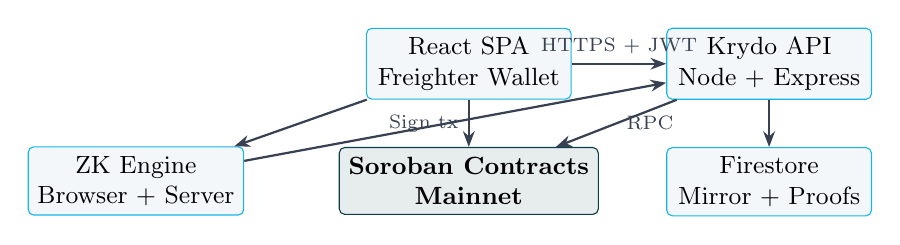
\begin{tikzpicture}[
    node distance=0.6cm and 1.2cm,
    box/.style={draw=StellarBlue, fill=LightBg, rounded corners=2pt,
                minimum width=2.6cm, minimum height=0.85cm, align=center, font=\small},
    chain/.style={draw=StellarDark, fill=StellarDark!10, rounded corners=2pt,
                  minimum width=3cm, minimum height=0.85cm, align=center, font=\small\bfseries},
    arr/.style={-{Stealth[length=2mm]}, thick, color=BodyGray}
  ]
    \node[box] (client) {React SPA\\Freighter Wallet};
    \node[box, right=of client] (api) {Krydo API\\Node + Express};
    \node[box, below=of api] (db) {Firestore\\Mirror + Proofs};
    \node[chain, below=of client] (soroban) {Soroban Contracts\\Mainnet};
    \node[box, left=of soroban] (zk) {ZK Engine\\Browser + Server};

    \draw[arr] (client) -- node[above, font=\scriptsize] {HTTPS + JWT} (api);
    \draw[arr] (client) -- node[left, font=\scriptsize] {Sign tx} (soroban);
    \draw[arr] (api) -- (db);
    \draw[arr] (api) -- node[right, font=\scriptsize] {RPC} (soroban);
    \draw[arr] (client) -- (zk);
    \draw[arr] (zk) -- (api);
  \end{tikzpicture}
  \caption{\krydo{} on \stellar{} --- high-level architecture}
\end{figure}

\subsection{Post-Residency Technical Debt}

\begin{enumerate}
  \item On-chain \soroban{} ZK verifier (Groth16/PLONK) for trustless verification
  \item Ed25519-native Pedersen commitments (full cryptographic port from secp256k1)
  \item Multi-sig root authority and decentralised issuer governance
  \item Third-party cryptographic audit before regulated financial production use
  \item SOC-2 equivalent backend certification
\end{enumerate}

% ═════════════════════════════════════════════════════════════════════════════
\section{Demo Day Strategy (25 July 2026)}

\subsection{Three-Act Live Demo Script (5--7 Minutes)}

\begin{enumerate}
  \item \textbf{Act 1 --- Trust Setup (60 sec):} Show whitelisted issuer on \stellar{} mainnet explorer. Explain Root Authority $\rightarrow$ Issuer trust chain.
  \item \textbf{Act 2 --- Credential + Proof (2 min):} Issue income credential; user generates ZK proof in browser; show commitment math briefly (optional slide).
  \item \textbf{Act 3 --- Verification (2 min):} Lender scans QR / enters proof ID; API returns \texttt{valid: true, reason: ``income $\geq$ INR\,10\,Lakh''}; emphasise actual salary never transmitted.
  \item \textbf{Close (60 sec):} Business model, India DPDP angle, pilot ask, \stellar{} cross-border vision.
\end{enumerate}

\subsection{Pitch Deck Structure (Recommended Slides)}

\begin{enumerate}
  \item Title + one-liner
  \item Problem: over-collection in Indian verification
  \item Solution: \krydo{} four-actor model + live demo screenshot
  \item Why ZK (not fake privacy): sigma protocols, on-chain anchor
  \item Why \stellar{}: cost, speed, cross-border, Rise In support
  \item Business model: who pays, unit economics, INR worked example
  \item Market: NBFC/fintech wedge, DPDP tailwind
  \item Traction plan: residency demo, LOI targets, 90-day pilot
  \item Team
  \item Ask: pilot intros, mainnet sponsorship confirmation, SCF pathway
\end{enumerate}

\subsection{Backup Plan}

\begin{itemize}
  \item Pre-recorded demo video (2 min) if live network fails
  \item Testnet fallback environment with mainnet addresses shown separately
  \item Printed QR codes tested 24 hours before pitch
\end{itemize}

% ═════════════════════════════════════════════════════════════════════════════
\section{Financial Projections (Directional)}

\subsection{Year 1 P\&L Summary (Conservative Scenario)}

\begin{table}[H]
  \centering
  \caption{Year 1 financial outlook (INR, conservative)}
  \renewcommand{\arraystretch}{1.2}
  \begin{tabular}{@{}lrr@{}}
    \toprule
    \textbf{Line Item} & \textbf{Year 1} & \textbf{Notes} \\
    \midrule
    Revenue --- pilot contracts & 6,00,000 & 2--3 paid pilots \\
    Revenue --- API subscriptions & 18,00,000 & 4--6 verifier clients \\
    Revenue --- issuer onboarding & 4,00,000 & 1--2 issuers \\
    \midrule
    \textbf{Total Revenue} & \textbf{28,00,000} & \\
    \midrule
    Infrastructure (Render, Firebase, RPC) & 1,20,000 & \\
    \stellar{} mainnet transaction costs & 30,000 & Subsidised early stage \\
    Team (founders + 1 contractor) & 18,00,000 & Lean team \\
    Legal \& compliance & 2,00,000 & \\
    Sales \& marketing & 1,50,000 & \\
    \midrule
    \textbf{Total Costs} & \textbf{23,00,000} & \\
    \midrule
    \textbf{Net (pre-grant)} & \textbf{5,00,000} & SCF grant extends runway \\
    \bottomrule
  \end{tabular}
\end{table}

\subsection{Funding Strategy}

\begin{enumerate}
  \item \textbf{Immediate:} \stellar{} Garage mainnet sponsorship (in-kind)
  \item \textbf{Month 2--4:} SCF Build Award application (USD\,50--150K range, directional)
  \item \textbf{Month 6+:} Angel/pre-seed from fintech-focused angels (INR\,50L--1.5Cr) post-pilot traction
  \item \textbf{Avoid:} Raising before first paid pilot---LOI + pilot revenue de-risks valuation
\end{enumerate}

% ═════════════════════════════════════════════════════════════════════════════
\section{Risk Analysis \& Mitigation}

\begin{table}[H]
  \centering
  \caption{Risk register}
  \renewcommand{\arraystretch}{1.25}
  \small
  \begin{tabularx}{\textwidth}{@{}>{\bfseries}p{2.5cm} p{1.2cm} X X@{}}
    \toprule
    Risk & Severity & Impact & Mitigation \\
    \midrule
    ZK crypto port delays & High &
    Mainnet demo scope creep &
    Keep proofs off-chain; anchor hashes on \soroban{} only for MVP \\

    21-day timeline insufficient & High &
    Incomplete mainnet deploy &
    Ruthless scope cut; pre-built Ethereum demo as fallback narrative \\

    No paying customers post-residency & Medium &
    Revenue gap &
    LOI outreach during residency; 90-day paid pilot offer \\

    Regulated entity sales cycle & Medium &
    Slow revenue &
    Start with crypto exchanges and PropTech (faster procurement) \\

    Backend ZK verifier trust & Medium &
    Enterprise objection &
    Roadmap on-chain verifier; third-party audit plan \\

    Issuer adoption chicken-and-egg & Medium &
    Empty credential network &
    Sandbox/mock issuers for pilot; partner with one payroll SaaS \\

    Mainnet deploy failure on pitch day & Low &
    Program disqualification &
    Deploy by 23 July; 48-hour buffer; recorded backup demo \\
    \bottomrule
  \end{tabularx}
\end{table}

% ═════════════════════════════════════════════════════════════════════════════
\section{Competitive Moat \& Defensibility}

\begin{enumerate}
  \item \textbf{Trust network ownership:} Root Authority controls issuer whitelist---credentials without \krydo{} approval are not trusted by the network.
  \item \textbf{Cryptographic implementation:} 154 tests, sigma protocol engine, Pedersen commitments---not a wrapper around basic hashing.
  \item \textbf{Dual-layer architecture:} On-chain truth (what exists, who issued) + off-chain performance (Firestore queries, proof storage).
  \item \textbf{Regulatory positioning:} First-mover narrative on DPDP-aligned data minimisation for Indian fintech.
  \item \textbf{\stellar{} ecosystem lock-in:} Early mainnet deployment + SCF relationship + cross-border use case development.
  \item \textbf{API-first distribution:} Embedded verification becomes infrastructure; high switching costs once integrated into loan origination flow.
\end{enumerate}

% ═════════════════════════════════════════════════════════════════════════════
\section{Conclusion \& Immediate Next Steps}

\krydo{} addresses a real, paid problem in India's verification infrastructure: \textbf{organisations need to know if someone qualifies; they do not need to own that person's entire financial identity.} Deploying on \stellar{} mainnet via the Stellar Garage Delhi residency provides the credibility, ecosystem access, and technical forcing function to convert a strong engineering MVP into a fundable B2B business.

\subsection{Immediate Action Items}

\begin{table}[H]
  \centering
  \renewcommand{\arraystretch}{1.2}
  \begin{tabularx}{\textwidth}{@{}>{\bfseries}p{0.5cm} X >{\bfseries}p{2.2cm}@{}}
    \toprule
    \# & Action & Deadline \\
    \midrule
    1 & Attend Build Station Day 1 kickoff at Innov8 CP & 4 Jul 2026 \\
    2 & Complete Soroban dev environment setup & 5 Jul 2026 \\
    3 & Deploy Authority contract to Stellar testnet & 7 Jul 2026 \\
    4 & End-to-end testnet demo (issue $\rightarrow$ prove $\rightarrow$ verify) & 10 Jul 2026 \\
    5 & Progress update with screen recording & Weekly \\
    6 & Rise In mainnet sponsorship confirmation & 11 Jul 2026 \\
    7 & Mainnet deployment & 22--23 Jul 2026 \\
    8 & Final pitch + live mainnet demo & 25 Jul 2026 \\
    9 & First paid pilot LOI signed & 31 Aug 2026 \\
    \bottomrule
  \end{tabularx}
\end{table}

\vspace{1em}
\begin{keybox}[Final Statement]
  \centering
  \large\textit{Prove you qualify --- without revealing what you have.}\\[0.4em]
  \normalsize \krydo{} on \stellar{} Mainnet \textbar\ Stellar Garage Delhi 2026
\end{keybox}

% ═════════════════════════════════════════════════════════════════════════════
\appendix
\section{Appendix A: API Endpoints (Reference)}

\begin{table}[H]
  \centering
  \small
  \renewcommand{\arraystretch}{1.15}
  \begin{tabularx}{\textwidth}{@{}ll X@{}}
    \toprule
    \textbf{Method} & \textbf{Endpoint} & \textbf{Purpose} \\
    \midrule
    POST & \texttt{/api/zk/generate} & Generate ZK proof from credential \\
    POST & \texttt{/api/zk/verify} & Verify proof; return predicate result \\
    GET & \texttt{/verify/:id} & Public verification page (QR target) \\
    POST & \texttt{/api/credentials/issue} & Issue credential (issuer role) \\
    GET & \texttt{/api/issuers} & List whitelisted issuers \\
    POST & \texttt{/api/auth/siwe} & Wallet authentication (Stellar adapt.) \\
    \bottomrule
  \end{tabularx}
\end{table}

\section{Appendix B: Progress Update Template}

\begin{verbatim}
Week [N] Progress Update -- Krydo on Stellar
-------------------------------------------
Completed:
  - [Specific deliverable with screenshot/recording link]

Metrics:
  - Testnet transactions: [N]
  - API endpoints working: [list]
  - Tests passing: [N/N]

Next 3 Days:
  - [ ] Task 1
  - [ ] Task 2
  - [ ] Task 3

Blockers:
  - [None / describe and ask for help]
\end{verbatim}

\section{Appendix C: Document \& Resource Links}

\begin{itemize}
  \item Repository: \url{https://github.com/nishant-uxs/krydo}
  \item Stellar Documentation: \url{https://developers.stellar.org/}
  \item Soroban Smart Contracts: \url{https://soroban.stellar.org/}
  \item Stellar Community Fund: \url{https://communityfund.stellar.org/}
  \item Rise In: \url{https://risein.com/}
  \item Technical Documentation: \texttt{DOCUMENTATION.md} (project repository)
  \item Deployment Guide: \texttt{DEPLOY.md} (project repository)
\end{itemize}

\end{document}
